\documentclass[10pt,a4paper]{article} % Compila con lualatex o xelatex

% --- Layout & links ---
\usepackage[english]{babel}
\usepackage[margin=1.5in]{geometry}
\usepackage[hidelinks]{hyperref}

% --- Fuentes (texto y matemáticas) ---
\usepackage{amsmath}  % Para escribir fórmulas matemáticas
\usepackage{amssymb}  % Símbolos adicionales
\usepackage{fontspec}  % Para usar fuentes del sistema
\usepackage{newtxmath}  % Libertinus Math para fórmulas
\setmainfont{EB Garamond}[
  UprightFont = * Medium,
  ItalicFont = * Medium Italic,
  BoldFont = * SemiBold,
  BoldItalicFont = * SemiBold Italic
]

% --- Secciones y subsecciones ---
\usepackage{titlesec}
\newfontface\garamondbold{EB Garamond Bold}
\newfontface\garamondbolditalic{EB Garamond Bold Italic}
\titleformat{\section}
  {\garamondbold\Large}{\thesection}{1em}{}
\titleformat{\subsection}
  {\garamondbold\large}{\thesubsection}{1em}{}

% --- Encabezado con nombre de la sección ---
\usepackage{fancyhdr}
\pagestyle{fancy}
\fancyhf{}
\fancyhead[L]{\small\leftmark}
\fancyhead[R]{\small\thepage}
\renewcommand{\headrulewidth}{0.1pt}

% --- Espaciado ---
\usepackage{setspace}

% --- Otros paquetes útiles ---
\usepackage{tocloft}  % Para personalizar la tabla de contenidos
\usepackage{xcolor}   % Para colores en el código
\usepackage{booktabs} % Para tablas bonitas

% \usepackage{amsmath}
% \usepackage[colorlinks=true, allcolors=blue]{hyperref}

\usepackage{graphicx}

% --- Bibliografía ---
\usepackage{natbib}
\bibliographystyle{apalike}   % u otro: plainnat, abbrvnat, unsrtnat

% --- Código fuente ---
\usepackage{listings}
\lstset{
  basicstyle=\ttfamily\small,
  backgroundcolor=\color{gray!10},
  frame=single,
  breaklines=true
}

% interlineado de 1.2
\usepackage{setspace}
\setstretch{1.2}

\begin{document}

% --- Portada ---
\begin{titlepage}
  \centering
  \vspace*{4cm}
  {\Huge\bfseries Mexico Derivatives Market\par}
  \vspace{2cm}
  {\Large Heriberto Espino Montelongo\par}
  \vspace{1cm}
  {\large Universidad de las Américas Puebla\par}
  \vfill
  {\large \today\par}
\end{titlepage}

% --- Abstract ---
\begin{abstract}
This document provides a template for reports in the "AI in Financial Services" course, using EB Garamond for prose and Libertinus Math for formulas. It includes a cover page, abstract, table of contents, and sample sections for math and text. Additional content demonstrates tables, code, and references.
\end{abstract}

% --- Tabla de contenidos ---
\tableofcontents
\thispagestyle{empty}
\newpage


\section{Corn}


ZCZ5 Corn futures are vital to the agricultural commodities market, offering farmers, traders, and investors opportunities to hedge risks and speculate on price movements \citep{cme_corn_overview}. There are 13 elements that drive corn futures prices. Weather, supply and demand, ethanol production, government policies, global economic conditions, competing crops, transportation costs, storage costs and capacity, technological advancements, speculative trading, global events, and USDA reports and market information \citep{noaa_enso_discussion,ers_ethanol_40,ers_feedgrains_outlook,ams_gtr_2023,ncga_storage_2025,ers_precision_2023,cftc_cot_about,usda_wasde}. A brief overview of each one is that weather affects corn production, depending on the weather it can lead to supply shortages and price spikes \citep{noaa_enso_discussion}. Supply and demand refer to the basic economic principles. About 40\% of U.S. corn goes into ethanol production, therefore the renewable fuel industry influences corn prices \citep{ers_ethanol_40,ers_ethanol_2030}. Economic growth or recession impacts the demand and prices of corn \citep{ers_feedgrains_topic}. Competing crops refers to other crops like soybeans and their relative returns that may shift acreage away from corn \citep{ers_feedgrains_outlook}. Higher fuel prices can increase transport costs and corn prices \citep{ams_gtr_2023}. Limited storage capacity during harvests can pressure prices \citep{ncga_storage_2025}. Improvements in harvesting and precision-ag equipment may influence yields and cost structures \citep{ers_precision_2023}. Speculative trading can amplify moves; positioning is tracked in the CFTC Commitments of Traders reports \citep{cftc_cot_about,cftc_cot_notes}. Finally, monthly USDA WASDE and related reports anchor supply–demand expectations that reprice futures curves \citep{usda_wasde,usda_understanding_wasde}.



\begin{center}
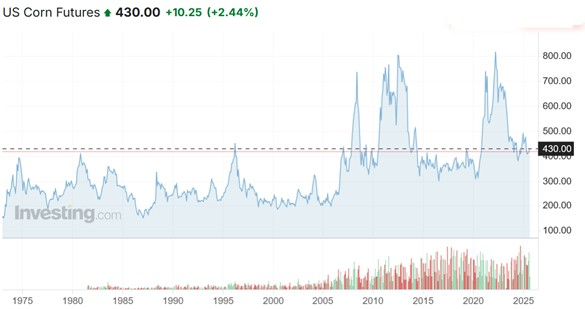
\includegraphics[width=0.5\textwidth]{figures/corn.jpg}
\end{center}

Mexico is structurally short yellow corn and imports most of it from the U.S., while white corn is central for tortillas. Policy has been in flux: Mexico's 2023 decree targeted biotech corn for human consumption and instructed a gradual substitution in other uses, triggering a USMCA dispute \citep{fas_mexico_decree_2023,ustr_usmca_biotech_2023}. In December 2024 the US prevailed at the USMCA panel \citep{ustr_usmca_biotech_win_2024}; Mexico has kept a domestic planting ban while adjusting import measures \citep{reuters_mexico_gm_ban_2025,fas_mexico_grain_annual_2025}. These shifts, together with U.S. supply and logistics, transmit into Mexican basis, feed costs, and tortilla inflation dynamics.

ZCZ5 denotes the CBOT Corn futures contract for December 2025 delivery (month code Z). Each contract is 5{,}000 bushels; tick size is $1/4$ cent per bushel (\$12.50 per contract) \citep{barchart_zc_specs}.
Recent U.S. balance-sheet news also matters: USDA has projected very large 2025 U.S. corn production, which weighs on deferred contracts like ZCZ5, all else equal \citep{reuters_record_crop_2025}.
% (Optional) Add a footnote if you want month codes spelled out.
\footnote{CBOT month codes: H=Mar, K=May, N=Jul, U=Sep, Z=Dec \citep{barchart_zc_specs}.}

\subsection{Pricing the ZCZ5 contract}
\begin{center}
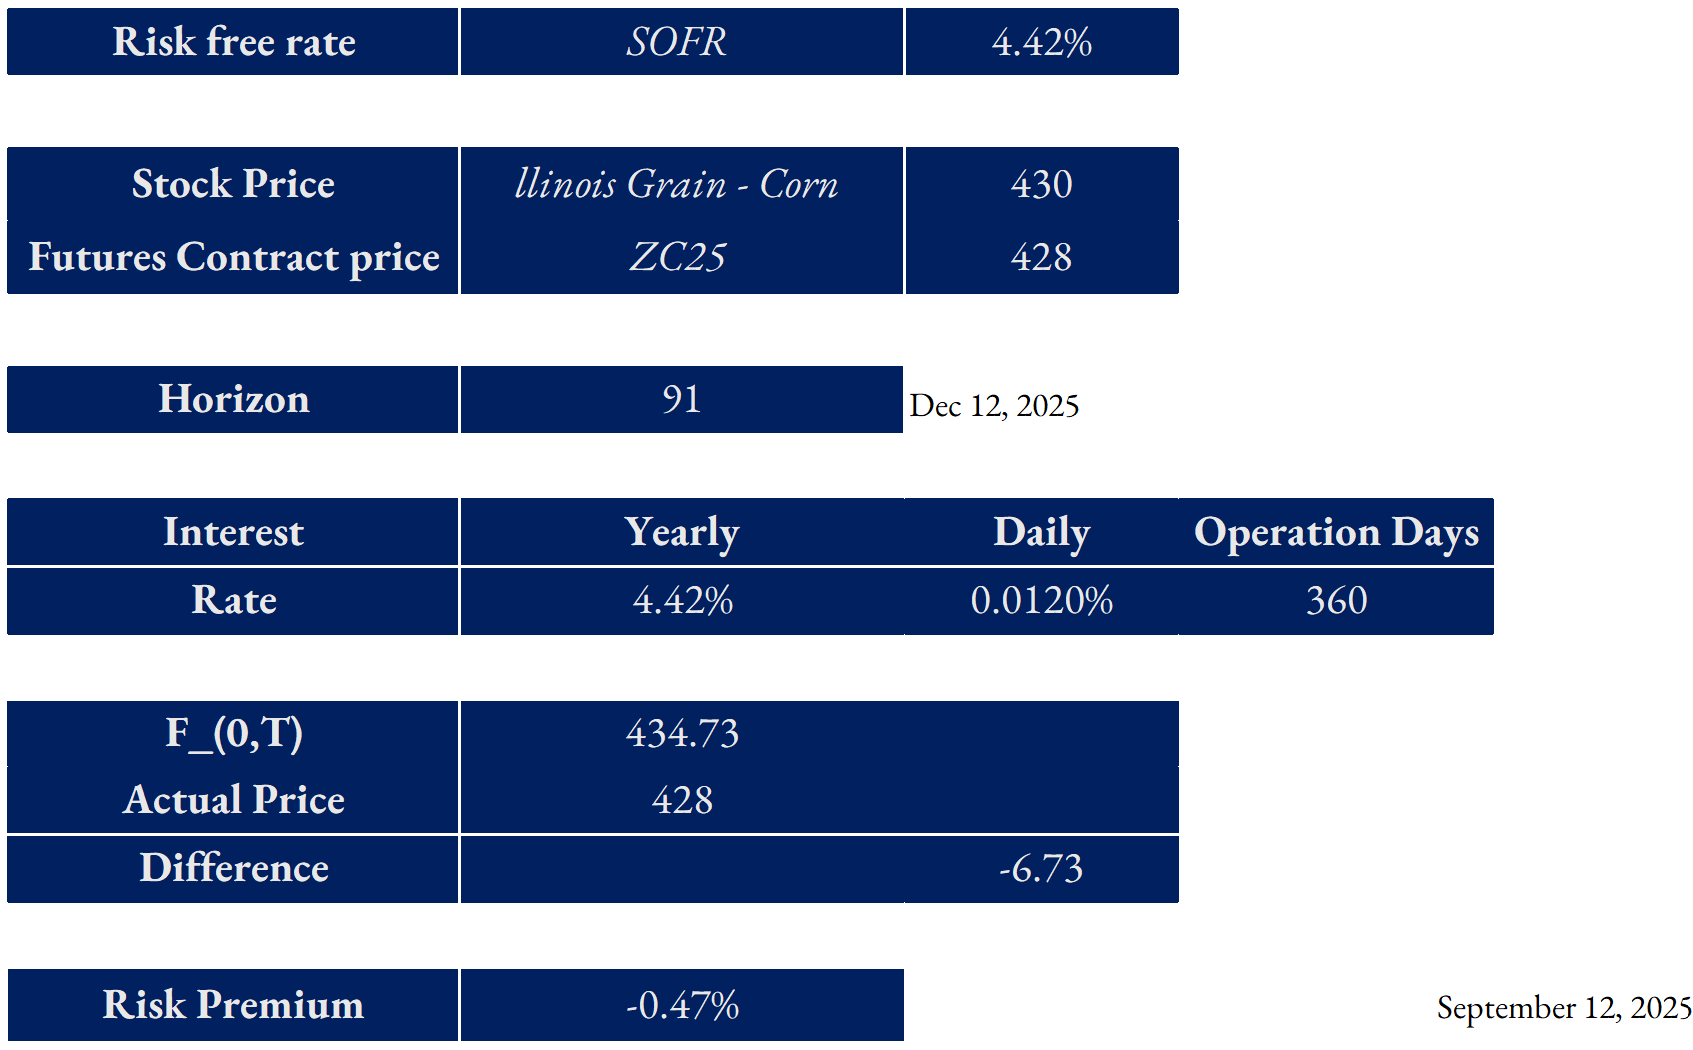
\includegraphics[width=0.5\textwidth]{figures/corn2.png}
\end{center}

A 91-day horizon (ACT/360) is used with $S=430.00$ ¢/bu for Illinois cash corn, $F=428.00$ ¢/bu for \textbf{ZCZ5}, and $r=4.41\%$. The no-carry fair value is obtained from $F^{\*}=S\,e^{rT}$, yielding
\[
T=\tfrac{91}{360},\quad F^{\*}=430\,e^{0.0441\cdot T}\approx \mathbf{434.72}\ \text{¢/bu}.
\]

A price difference of $\mathbf{-6.72}$ ¢/bu is observed $(F-F^{\*})$, which equals \textbf{26.9 ticks} and \textbf{\$336 per 5,000-bu contract}. The spot–futures return $F/S-1$ is $\mathbf{-0.47\%}$.

For interpretation, the cost-of-carry relation
\[
F=S\,e^{(r+u-y)T}
\]
is used, where $u$ represents storage and insurance costs and $y$ the convenience (or inventory) yield. The market carry is inferred as
\[
c_{\text{mkt}}=\frac{1}{T}\ln\!\frac{F}{S}
=\frac{1}{91/360}\ln\!\frac{428}{430}\approx \mathbf{-1.84\%}\ \text{per year}.
\]

It follows that the net convenience yield is obtained as
\[
y-u \approx r-c_{\text{mkt}}\approx 4.41\%-(-1.84\%)=\mathbf{6.25\%}\ \text{per year}.
\]

Therefore, a \textbf{negative basis} and $F<S e^{rT}$ are consistent with \textbf{backwardation}: near-dated corn is priced below pure financing carry because inventory availability, storage constraints, or location basis premia raise the value of holding physical grain now. The deviation is explained by $y$ and operational frictions, so it is interpreted as an inventory/logistics signal rather than a tradable arbitrage.


\section{Crude Oil}
Crude oil is one of the most important energy commodities, powering transportation, industry, and heating. Therefore, its price is influenced by a complex array of factors. One of the most significant is the balance between global supply and demand. During periods of strong economic growth, demand for oil increases due to higher transportation and manufacturing activity. Conversely, economic recessions can lead to a sharp drop in demand and lower prices \citep{eia_prices_2023}.

The decisions made by the Organization of the Petroleum Exporting Countries (OPEC) and its allies (OPEC+) are also a primary influence on oil prices. This group coordinates production levels among major oil-exporting nations. By restricting or increasing output, they can directly tighten or loosen global supply to stabilize or manipulate the market \citep{eia_opec_2024}.

Geopolitical events are a major source of price volatility. Conflicts, sanctions, or political instability in key oil-producing regions (like the Middle East, Russia, or Venezuela) can disrupt supply chains and threaten actual production, leading to fears of a shortage and spiking prices \citep{eia_prices_2023}.

Furthermore, fluctuations in the U.S. dollar significantly affect oil prices. Since oil is globally traded in U.S. dollars, a stronger dollar makes oil more expensive for countries using other currencies, which can dampen demand. A weaker dollar makes oil cheaper on international markets, potentially boosting demand \citep{bis_usd_commodity_2023,ecb_oil_usd_2024}.

In 2008, crude oil prices reached a historic peak. That July, the price of West Texas Intermediate (WTI) crude oil futures hit an all-time nominal high of \$147.27 per barrel. This surge was driven by a combination of robust global demand, geopolitical tensions, and significant financial speculation. From the start of 2007 to this peak, the price had increased by over 200\%. The subsequent crash later that year, as the global financial crisis crushed demand, demonstrates the extreme volatility of the oil market \citep{reuters_oil_peak_2008,worldbank_oil_spike_2008}.

\textbf{CLV25} refers to the WTI (West Texas Intermediate) crude oil futures contract that expires in October 2025. Each contract represents 1{,}000 barrels and is quoted in U.S. dollars (USD) per barrel \citep{cme_cl_specs,cme_cl_calendar}.
This table compares the spot price, \$62.69, with what the futures price “should” be over 10 days using the 4.41\% annual risk-free rate and assuming there are no extra costs/benefits such as dividends \citep{frbny_sofr}.

\begin{center}
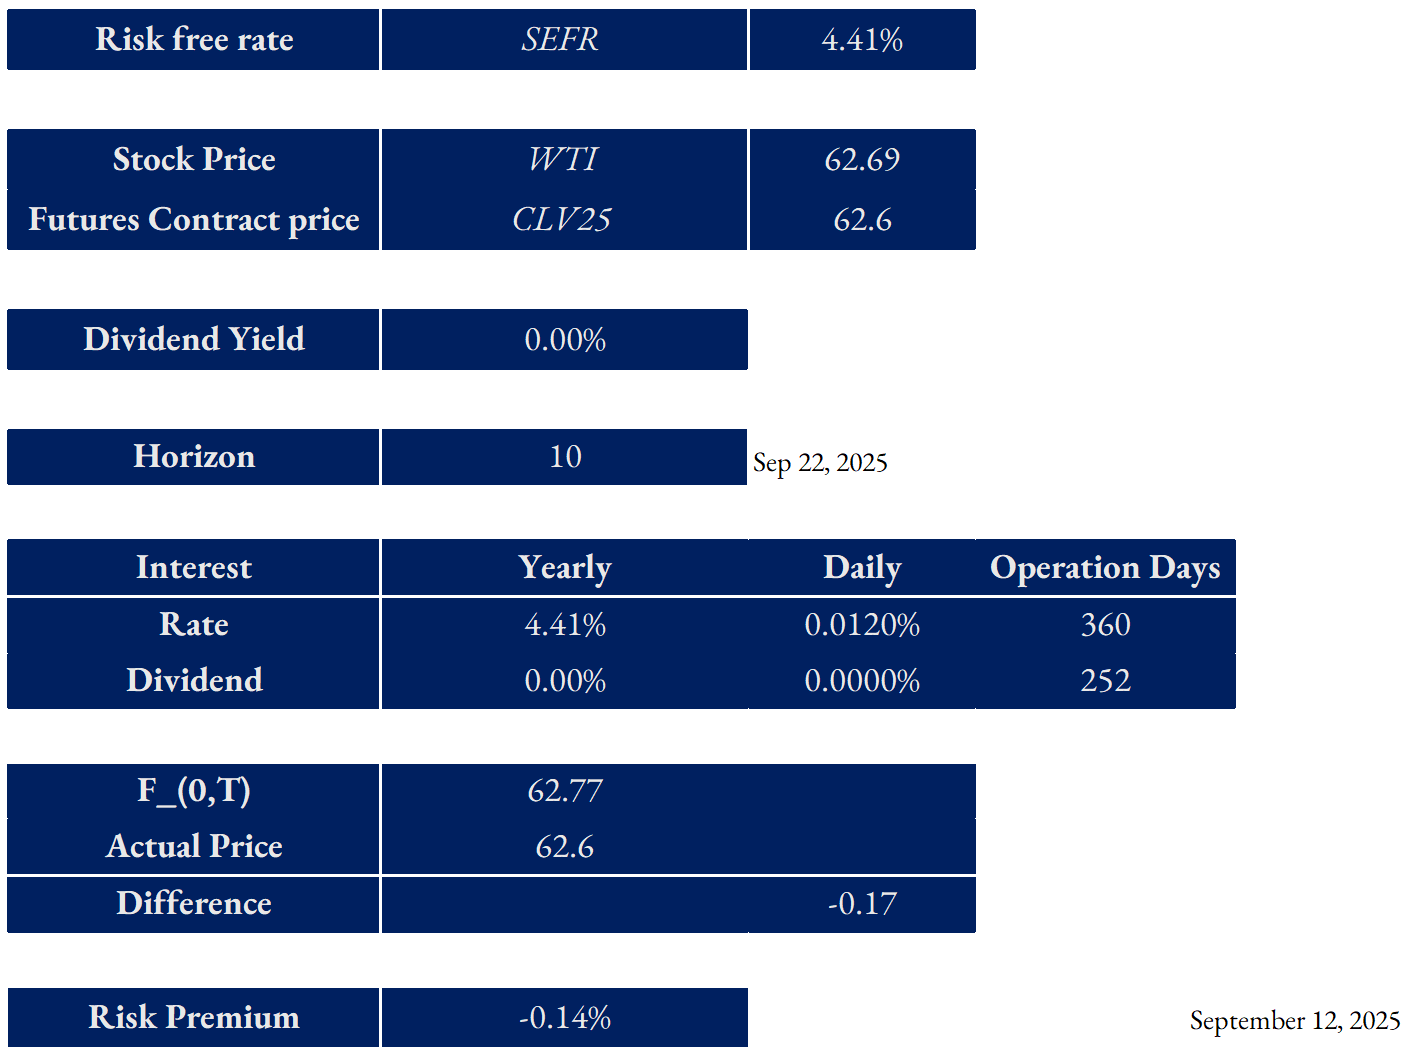
\includegraphics[width=0.5\textwidth]{figures/wti.png}
\end{center}

With those inputs, the theoretical price is computed as $F_{0,T} \approx S_0(1 + rT)$. For 10 days, $rT \approx 0.0441 \times \frac{10}{360} = 0.1225\%$. Therefore, $F_{0,T} \approx 62.69 \times (1 + 0.001225) = 62.77$. The market, however, is at 62.60. That means the actual futures price is \$0.17 per barrel below the theoretical value.

In percentage terms, the “risk premium” shown in the table is $-0.14\%$. That comes from comparing the futures price to spot: $62.60/62.69 - 1 \approx -0.14\%$. By contrast, the $-\$0.17$ difference you highlight is the gap between the market futures price and the theoretical futures price.

Economically, this discount indicates mild backwardation: the nearby contract is worth slightly less than what the interest rate alone would imply. In commodities like crude oil, this is often interpreted as an implicit convenience yield (the benefit of holding the physical now) that offsets the interest rate \citep{kaldor_working_brennan, eia_backwardation_2013, milonas_convenience_2024}. Roughly, the total deviation from the theoretical value is $\sim 0.2625\%$ over 10 days, which annualizes to about a $9.5\%$ convenience yield net of costs.

Practically speaking, for the standard contract size (1{,}000 barrels), that \$0.17 amounts to \$170 per contract \citep{cme_cl_specs}.


A 10-day valuation window is used with $S=62.69$, $F=62.60$, and $r=4.41\%$ (ACT/360). The no-carry fair value is computed as
\[
F^{\*}=S\,e^{rT}=62.69\,e^{0.0441\cdot(10/360)}\approx62.77.
\]

A price difference of
\[
-\$0.17
\]
per barrel is observed $(F-F^{\*})$, which corresponds to 17 ticks (\$170 per standard 1,000-barrel contract). In percentage terms, a spot–futures discount of
\[
\frac{F}{S}-1 \approx -0.14\%
\]
is obtained.

For interpretation, the cost-of-carry relation
\[
F=S\,e^{(r+u-y)T}
\]
is used, where $u$ denotes storage/insurance costs and $y$ denotes the convenience yield. The market carry is inferred as
\[
c_{\text{mkt}}=\frac{1}{T}\ln\!\frac{F}{S}\approx-5.17\%\ \text{per year},
\]
and the net convenience yield is obtained as
\[
y-u \approx r-c_{\text{mkt}}\approx 4.41\%-(-5.17\%)=9.6\% \ \text{per year}.
\]

Hence, the observed discount is consistent with \textbf{backwardation}: inventory is valued sufficiently highly (or storage is constrained) so that $y$ more than offsets financing $r$ and any $u$. No-arbitrage is preserved because $y$ and operational frictions are not directly tradable; the deviation is therefore read as a signal of tight near-term balances rather than a free arbitrage.



\section{Silver}
Silver has many uses, mainly in the industrial side. Therefore, there are many factors that influence its price. One of them is the global economy. Fluctuations in global growth or changes in monetary policies can impact demand for silver. Usually, during economic expansions, the demand for silver increases because of more manufacturing and technology. Fluctuations in currency can also affect demand for silver, especially talking about the US dollar. When the currency is stronger, the demand for silver is less because it is more expensive \citep{silver_institute_wss_2024,usgs_silver_mcs_2024,bis_usd_commodity_2023}.

\begin{figure}[h]
\centering
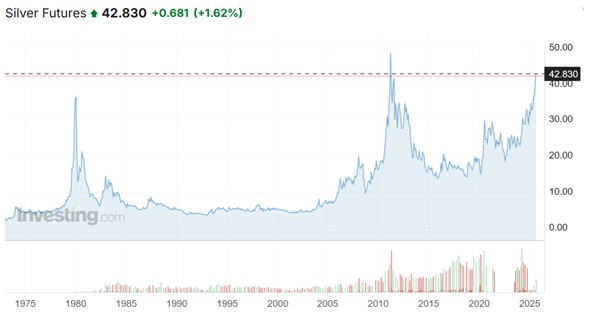
\includegraphics[width=0.7\textwidth]{figures/silver.jpg}
\caption{Silver price series. Source: Investing.com.}
\end{figure}

Geopolitical events are also an influence on silver prices. Trade policies, tariffs, or tensions between nations can affect the supply chains and international trade that impact its availability and price \citep{silver_institute_wss_2024}.

In 1980 there was a big high in silver futures. That event is known as Silver Thursday, and it referred to the Thursday 27th of March 1980 \citep{britannica_silver_thursday,nyt_1980_silver_thursday}.


\begin{figure}[h]
\centering
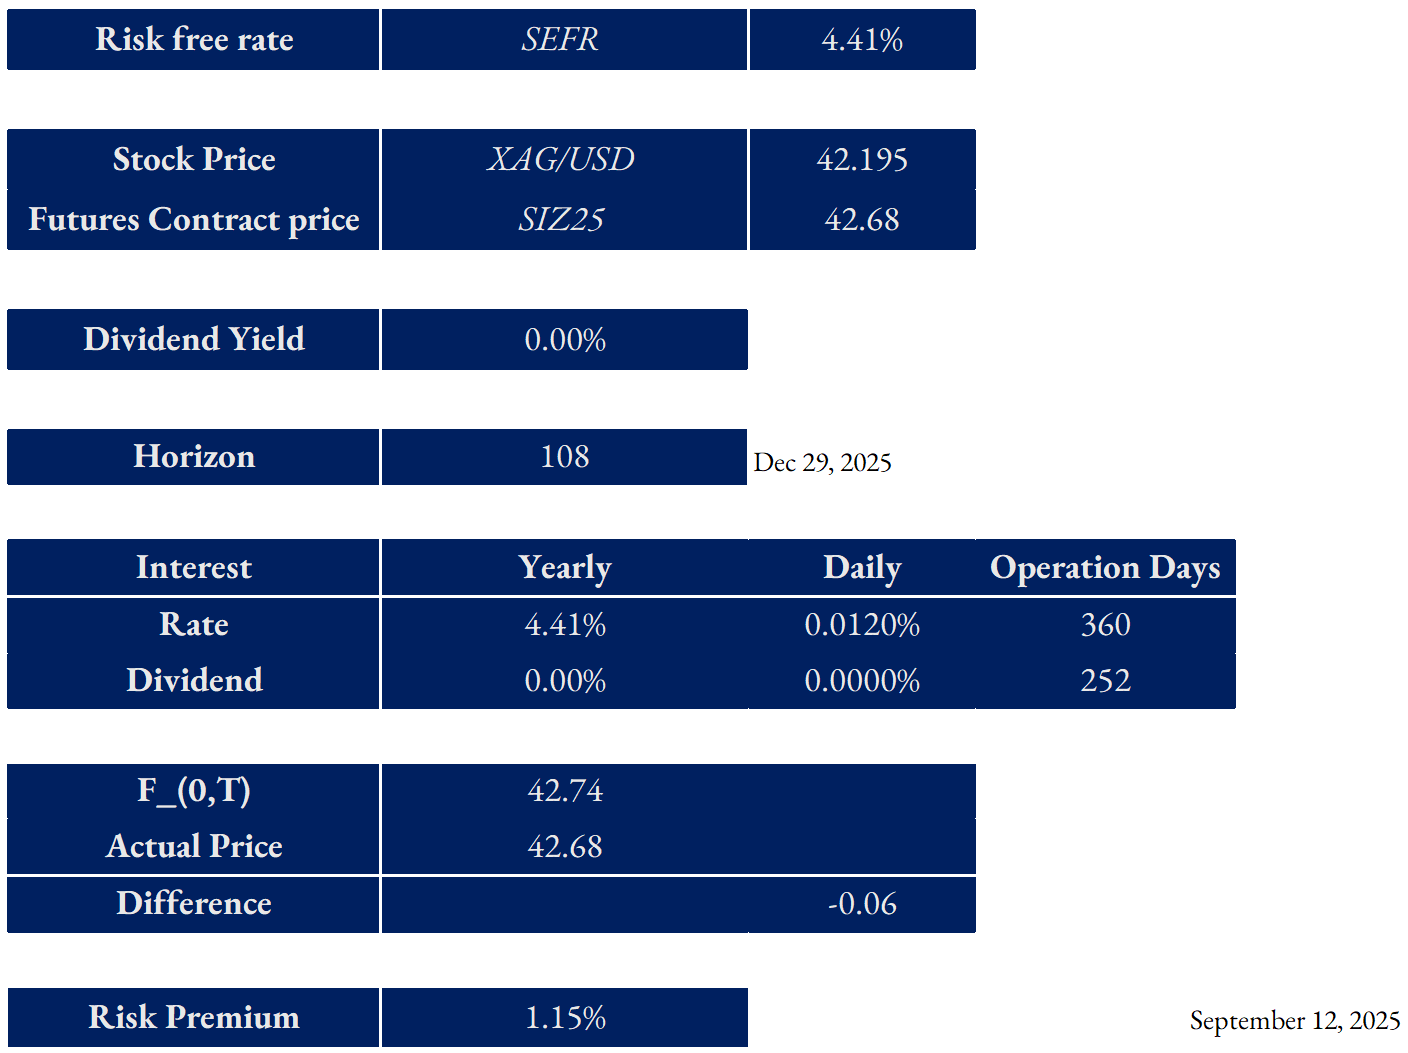
\includegraphics[width=0.7\textwidth]{figures/silver2.png}
\caption{Silver price series. Source: Investing.com.}
\end{figure}


\section{MXN/USD}
The exchange rate of the Mexican Peso (MXN) against the US Dollar (USD) is a crucial indicator of the Mexican economy and is influenced by a complex mix of domestic and international factors. One of the most important is the monetary policy of the US Federal Reserve (Fed). When the Fed raises its interest rates, the dollar strengthens, attracting investment into dollar-denominated assets and commonly causing a depreciation of the peso (i.e., it takes more pesos to buy one dollar). Similarly, interest rate decisions by the Bank of Mexico (Banxico) impact the exchange rate; higher rates can strengthen the peso by attracting foreign investment \citep{dallasfed_peso_2023,banxico_regional_2024}.

The overall state of the worldwide economy and investors' willingness to engage in risk are also pivotal determinants. The MXN is considered a "risk currency" or an "emerging market currency." During periods of global optimism and stability, investors often seek higher returns in emerging markets like Mexico, which appreciates the peso. Conversely, in times of uncertainty, geopolitical tension, or global recessions, investors seek safe-haven assets like the US dollar, triggering a massive sell-off of pesos and its depreciation \citep{bis_eme_internationalisation_2022}.

Internal factors and Mexico's economic situation play a fundamental role. Macroeconomic data such as GDP growth, the unemployment rate, inflation, and consumer confidence affect the perception of the country's stability. Furthermore, political events like elections, changes in fiscal policy (budgets, taxes), or the implementation of structural reforms can generate volatility in the exchange rate by impacting the confidence of foreign investors \citep{banxico_regional_2024}.

A historical event that exemplifies the MXN's extreme volatility was the Tequila Crisis in 1994. In December of that year, the Mexican government was forced to devalue the peso, which in a matter of days went from a fixed exchange rate of approximately 3.50 MXN per USD to over 7.00 MXN per USD—a devaluation of over 100\%. This crisis was triggered by a combination of a current account deficit, capital flight, and a crisis of confidence in economic policy \citep{imf_tequila_2012,yale_tequila_2012}.


\textbf{MPZ25} refers to the Mexican peso futures contract (MXN/USD quoted in \text{USD per 1 MXN}) that expires in December 2025. The current contract price shown is \(0.0537\) USD per MXN (equivalent to \(\sim 18.62\) MXN per USD). The spot used in the table is \(0.054266721\) USD per MXN (\(\sim 18.43\) MXN per USD) \citep{cme_mxn_product,cme_mxn_rulebook}.

This table compares the spot with what the futures price “should” be over \(94\) days using a USD risk-free rate (SEFR) of \(4.41\%\) and no extra costs/benefits. With those inputs, the theoretical price would be \(F_{0,T} \approx S_0(1+rT)\). For \(94\) days, \(rT \approx 0.0441 \times \frac{94}{360} = 0.01152\). Then \(F_{0,T} \approx 0.054266721 \times (1+0.01152) \approx \mathbf{0.05489}\) \citep{frbny_sofr}.\footnote{SEFR is commonly referred to as SOFR; data and methodology: \citep{frbny_sofr,frbny_sofr_index}.}
The market, however, is at \(0.0537\). This implies the futures price is \(0.00118\) below the theoretical value (\(\approx -2.17\%\) relative to that calculation).

In percentage terms versus spot, the table reports a “risk premium” of \(-1.04\%\), which comes from \(0.0537/0.054266721 - 1 \approx -1.04\%\).
The fair forward in FX follows covered interest parity: \(F \approx S_0 \frac{1 + r_{\text{USD}} T}{1 + r_{\text{MXN}} T}\) \citep{bis_cip_2016,bis_cip_2024}.

Since MXN rates are usually higher than USD rates, the MXN/USD forward is normally below the spot (i.e., the USD is expected to be more expensive in the future), which is exactly what your table shows. For example, if you assume an MXN rate around \(10\%\) annually for that tenor, the theoretical price is approximately \(F \approx 0.05427 \times \frac{1 + 0.0441 \cdot 94/360}{1 + 0.10 \cdot 94/360} \approx 0.0535\), very close to the \(0.0537\) in the market \citep{bis_cip_2016}.

\begin{figure}[h]
\centering
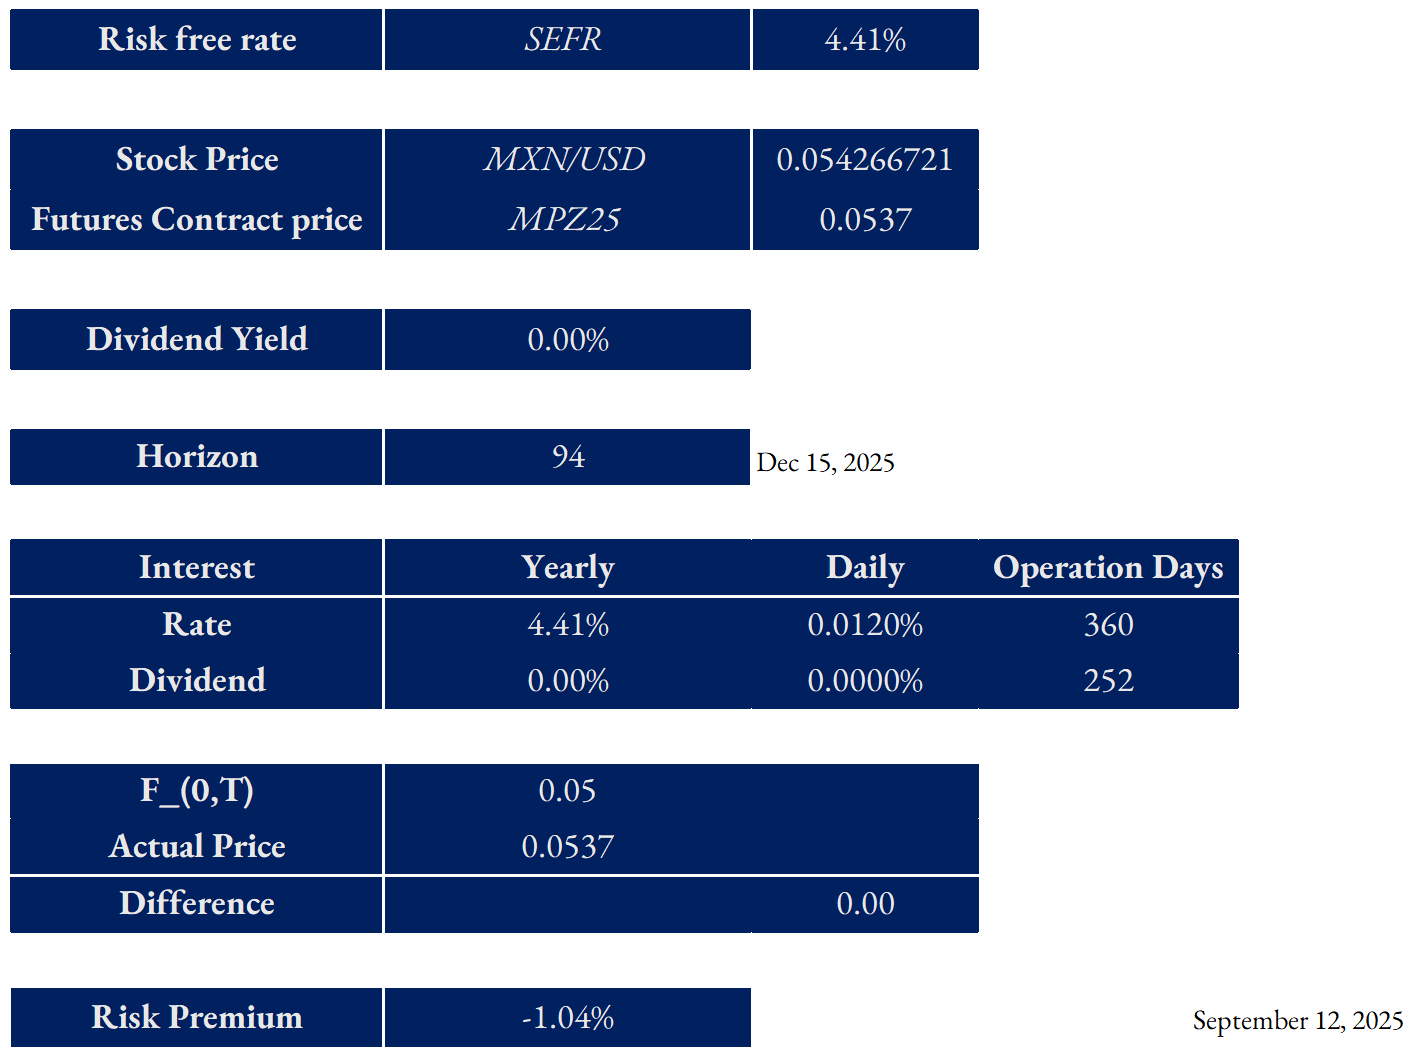
\includegraphics[width=0.7\textwidth]{figures/usdmxn.png}
\caption{Silver price series. Source: Investing.com.}
\end{figure}



\newpage
\section{TIIE}


The TIIE is today the central reference for the cost of overnight peso funding; it is the base price of money used by banks and firms to set interest on loans, bonds, and other instruments. It is estimated with one-day wholesale repo operations settled at INDEVAL, with government or equivalent collateral, and with banks and broker-dealers as participants. Based on these transactions, Banxico reports a representative daily rate and, in addition, \textbf{composition indices} that accumulate daily factors over business or calendar days and ``forward compounded'' versions useful for contracts that require explicit capitalization. The result reflects what actually happened in the market \citep{banxico_methodology,banxico_indices}.

At the CME, the futures contract allows trading the compounded rate; by convention it is quoted as \textbf{Index = 100 - 100R}. For example, today the rate is 8.0126\% and its CME futures price for the TIEU25 contract maturing on September 30, 2025 is 92.28. 

\begin{center}
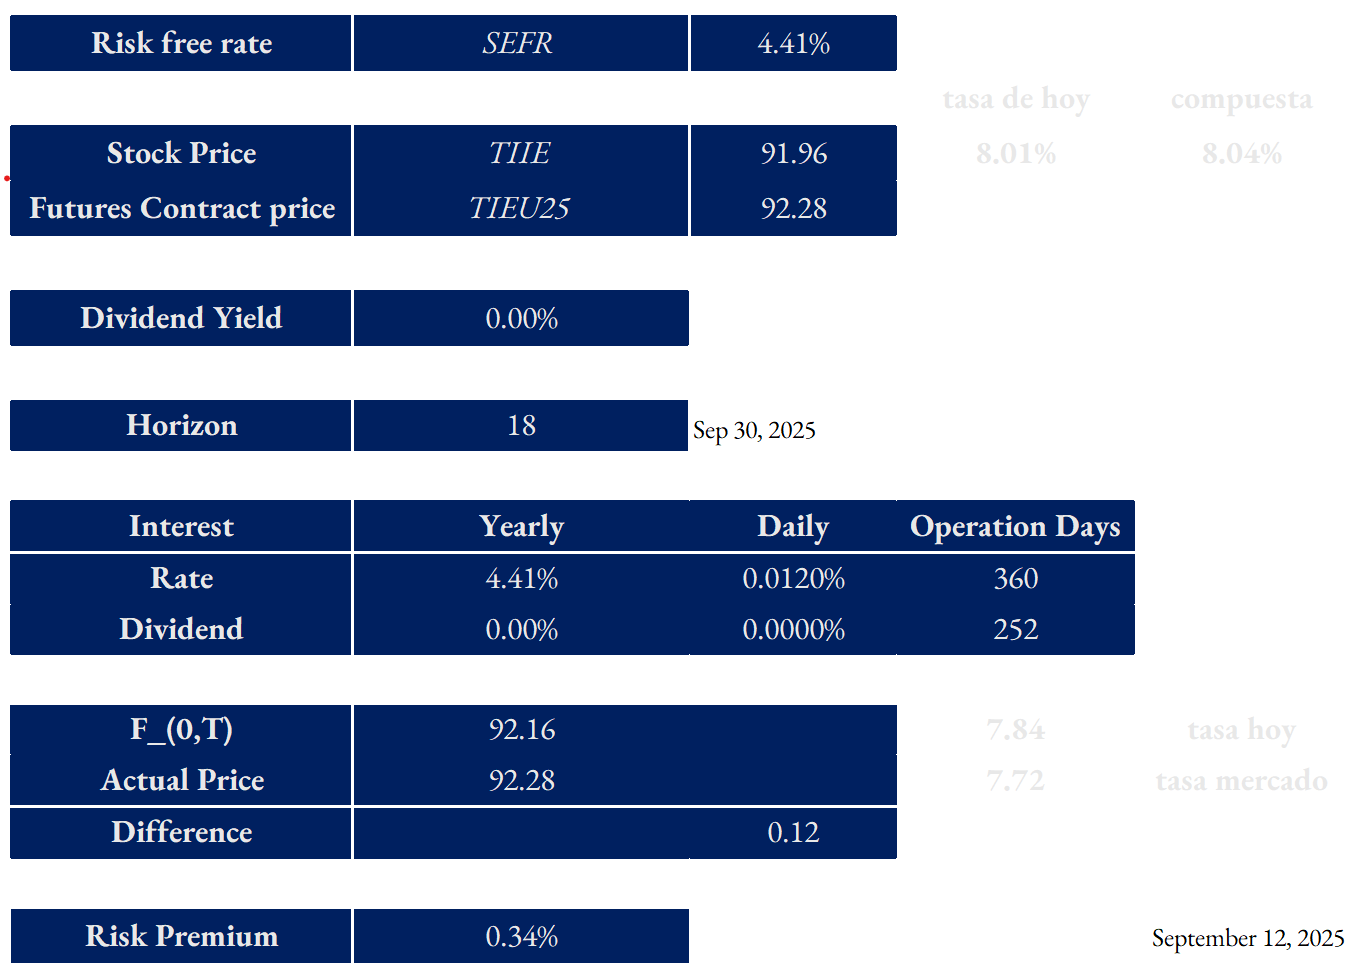
\includegraphics[width=0.5\textwidth]{figures/tiie.png}
\end{center}

A \textbf{positive basis in price} is observed: the \textbf{futures contract} $F=92.28$ is \textbf{above} the theoretical fair value $F^*=92.16$. The \textbf{implied monthly market rate} is therefore about \textbf{12 bps lower} than the model rate, since the market is discounting a \textbf{lower average TIEU25} for the remainder of the month than assumed by the fair value that is, a smoother downward path of rates. In other words, the expectation is for average rates to drift lower. Under the futures convention \textbf{Index = 100 - 100·R}, a \textbf{higher price implies a lower implied rate}. 

From this perspective, the market is effectively pricing a rate of:
\begin{itemize}
  \item \textbf{Market-implied}: $R_{\text{mkt}} = \tfrac{100-92.28}{100} = \mathbf{7.72\%}$.
  \item \textbf{Model (fair)}: $R_{\text{mod}} = \tfrac{100-92.16}{100} = \mathbf{7.84\%}$.
\end{itemize}

\textbf{Current level} (spot TIIE 28d $\approx 8.01\%$): since 12 days have already accrued at $\sim8.01\%$ and 18 days remain, in order for the monthly average to settle at $7.72\%$, the remaining path must evolve near \textbf{7.49\%}. This indicates a market signal of \textbf{gradual softening} of the TIEU25 for the rest of the month.

It is important to emphasize that this reflects an \textbf{expectation of the monthly average}, not a guarantee of an immediate policy cut. The 7.72\% already incorporates carry and the days elapsed; it may be achieved through a steady mild decline or fluctuations around $\sim7.5$--$7.6\%$. If the basis were negative (price $<$ fair), the interpretation would be reversed: an \textbf{implicit rise} in the expected average.

This could be caused by the fact that the Federal Reserve (Fed) is considering rate cuts because the labor market shows signs of cooling, with job creation revised down and unemployment slightly higher, which reduces wage and aggregate demand pressures \citep{reuters2025a}. In addition, inflation, while still above 2\%, shows some moderation and anchored expectations, which allows room for maneuver without eroding credibility \citep{ycharts2025}. At the same time, the policy rate remains in restrictive territory, above neutral, creating the risk of excessive slowdown \citep{ycharts2025}. Moreover, the U.S. economy faces stagnation signals and weaker growth, while the global environment increases vulnerabilities \citep{reuters2025b}. Finally, institutions such as the IMF have noted that the Fed has space to ease its stance given the deterioration in labor dynamics \citep{reuters2025c}, and Powell himself has acknowledged employment risks as an argument to open the door to cuts \citep{reuters2025d}.

If the Fed starts cutting and the peso remains stable, the market usually anticipates that the rate $R$ will decline; then the TIIE futures price rises. The approximate profit or loss per contract is 
\[
\Delta \text{P\&L} \approx 50{,}000 \times \Delta \text{Index} \quad \text{MXN}
\]
\citep{banxico2023,cme2025a,cme2025b,reuters2025a}. 

The process can be described as follows:

\begin{enumerate}
    \item New information arrives. For example, lower inflation signals in the U.S. and Fed guidance toward \textbf{consecutive cuts} \citep{reuters2025}.
    \item Very short-term USD rates fall. Dollar funding becomes cheaper and the expected path shifts downward.
    \item Global financial conditions ease. Lower risk aversion and often a weaker USD reduce imported inflationary pressure in Mexico.
    \item Banxico assesses the local picture. If inflation and the exchange rate cooperate, the market anticipates local cuts with a \textbf{lag} relative to the Fed. That \textbf{expected path} is what matters for derivatives.
    \item The expected TIEU25 for the quarter decreases. The compounded TIEU25 of the period, $R$, falls if each daily ``drop'' is slightly smaller.
    \item The futures price rises. By convention, \textbf{lower $R \Rightarrow$ higher Index}, because Index $= 100 - R$. A change of $-25$ bp in $R$ implies $+\!0.25$ index points.
\end{enumerate}

As an example, suppose the market expects an annualized compounded rate of $R = 10.00\%$. The futures contract trades near $100 - 10.00 = 90.00$. If, after cut guidance, consensus shifts to $R = 9.75\%$, the price would be 90.25. The approximate variation for a long contract is:

\[
\Delta \text{P\&L} \approx (90.25 - 90.00)\times 50{,}000 = \textbf{12{,}500 \ \text{MXN}}.
\]

Of course, this is not always the case, for several reasons:

\begin{itemize}
    \item \textbf{Local decoupling.} A rebound in Mexican inflation or a peso depreciation may lead Banxico to delay or cut less; $R$ falls less and the futures price rises less or corrects.
    \item \textbf{Technical factors.} Term premiums, paper supply, repositioning, or calendar effects. The compounding methodology extends the last published rate on weekends and holidays, introducing small differences across months and quarters and a \textbf{basis} between what you want to hedge and what the contract settles \citep{cme2025a,cme2025b}.
\end{itemize}



\section{IPC}

The S\&P/BMV IPC is the flagship index of the Mexican equity market, designed to measure the performance of the largest and most liquid stocks listed on the Bolsa Mexicana de Valores (BMV). It is float-adjusted, market-cap weighted, and maintained under published rules with regular rebalances \citep{spdj_ipc_page,spdj_bmv_methodology}.

\paragraph{Derivatives and implementation.}
Exposure and hedging are available via IPC futures listed at MexDer; these contracts are designed to manage equity-market risk tied to the Mexican market benchmark \citep{mexder_ipc_fut}.

\paragraph{Nowcasting the next move: macro–market linkages.}
As of \emph{September 12, 2025}, the IPC printed a new all-time high near 61{,}900, supported by risk-on flows as markets price imminent Fed cuts; the peso hovered around 18.4 per USD \citep{reuters_ipc_record_2025,reuters_usdmxn_quote}. This backdrop interacts with Mexico’s local cycle and policy mix:

\begin{enumerate}
    \item \textbf{Fed trajectory and global risk appetite.} Rising odds of a September Fed cut lowered U.S. yields and improved EM risk sentiment, historically supportive for Mexico’s equities and currency \citep{reuters_ipc_record_2025}.
    \item \textbf{Banxico path and inflation.} Recent data show headline inflation ticking up, prompting a slower easing cadence even as inflation expectations remain near target; net effect: supportive discount-rate impulse, but gradual \citep{bloomberg_mx_inflation_2025,mnd_inflation_band_2025}.
    \item \textbf{Fiscal stance and sovereign risk.} The 2026 budget narrative points to a slightly narrower deficit after 2025, with attention on execution and quasi-sovereign exposures (e.g., Pemex) that shape risk premia and equity multiples \citep{reuters_budget_2025,reuters_pemex_plan_2025}.
    \item \textbf{Trade/industrial policy shocks.} Proposed 50\% tariffs on vehicles from non-FTA countries would rewire EV/auto pricing in Mexico, with potential rotation across consumer, industrial, and materials names via supply-chain and price-elasticity channels \citep{reuters_tariffs_china_autos_2025}.
    \item \textbf{Nearshoring vs.\ frictions.} The medium-term nearshoring thesis coexists with cyclical frictions; recent reports of border-maquiladora job losses tied to U.S. tariff dynamics illustrate downside risk to industrial earnings momentum \citep{reuters_border_jobs_2025}.
\end{enumerate}

\paragraph{Base case and risks.}
Netting these forces, the near-term base case is a \emph{carry-and-liquidity-supported drift} while the Fed turns, tempered by Banxico’s gradualism and policy noise. Upside risks: faster global disinflation and credible domestic fiscal/Pemex execution that compress risk premia. Downside risks: renewed inflation pressure, sharper USD strength, escalation of tariff frictions, or disappointing growth that erodes earnings leverage \citep{reuters_ipc_record_2025,bloomberg_mx_inflation_2025,reuters_budget_2025,reuters_pemex_plan_2025,reuters_tariffs_china_autos_2025}.

\begin{figure}[h]
\centering
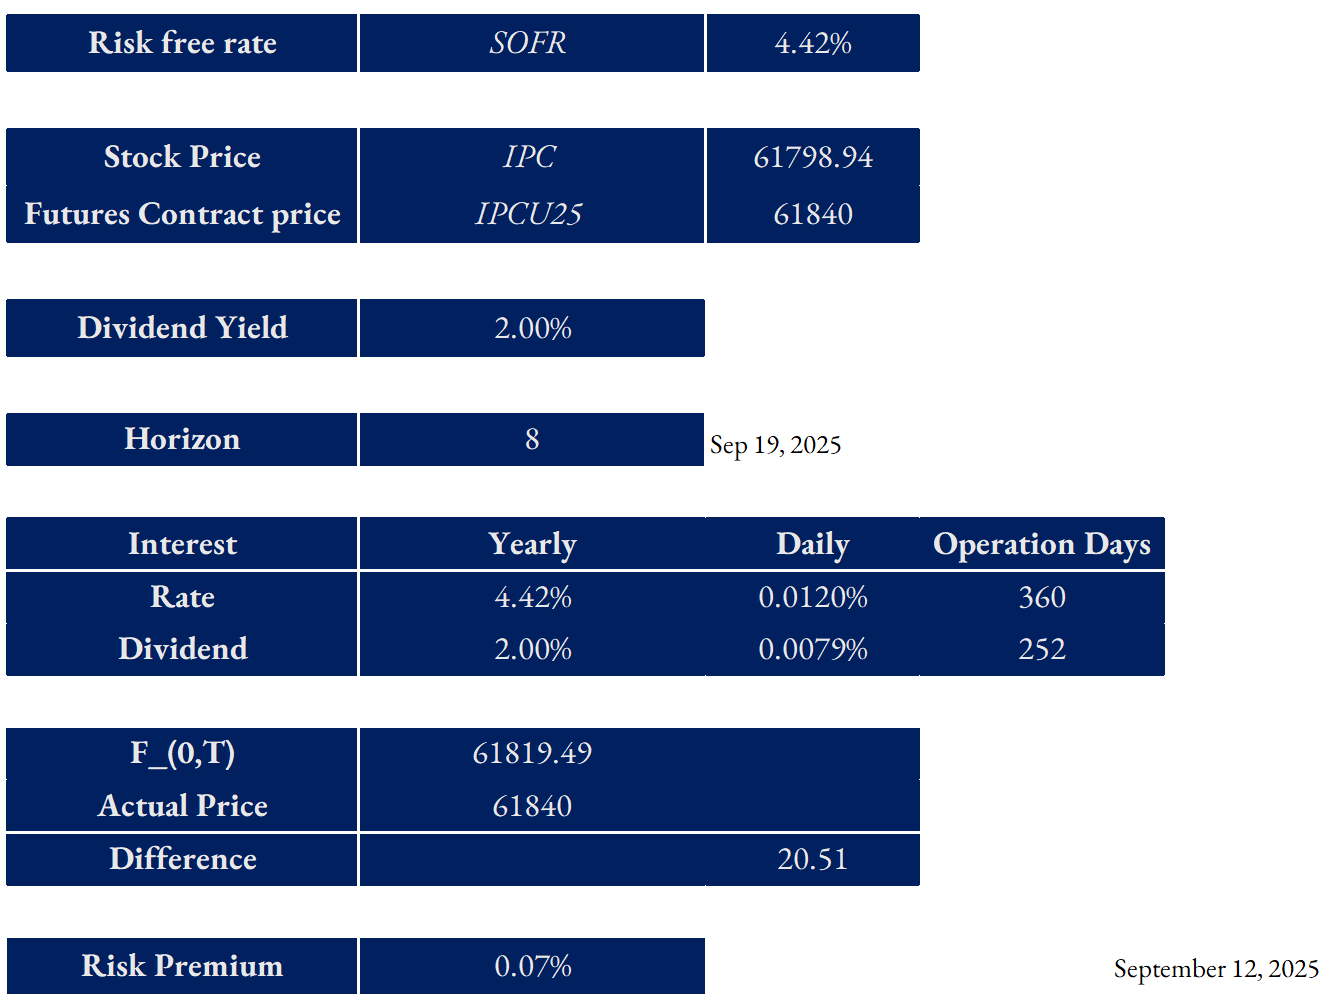
\includegraphics[width=0.7\textwidth]{figures/ipc.png}
\caption{Silver price series. Source: Investing.com.}
\end{figure}



\section{REFERENCIAS}


\bibliography{refs}



\end{document}